\documentclass{article}
\usepackage[margin=1in]{geometry}
\usepackage[utf8]{inputenc}
\usepackage{graphicx} 
\usepackage{fancyhdr}
\usepackage{enumitem}
\usepackage{lipsum}
\usepackage[bahasa]{babel}
\usepackage{subcaption}
\usepackage{float}
\usepackage{indentfirst}
\usepackage{listings}

\title{Laporan Workshop Telematika \\ ESP8266 Minimum System} % Ganti sesuai modul praktikum yang diikuti
\author{Azaria Putri Fawnia \\ 5024221038} % Ganti dengan NRP dan Nama Kalian

\date{}


\fancypagestyle{firstpageheader}{
  \fancyhf{} 
  \fancyhead[L]{
\includegraphics[height=1.5cm]{img/modul_1/logodepart.png}} 
  \fancyhead[R]{Institut Teknologi Sepuluh Nopember \\ Departemen Teknik Komputer \\ Laboratorium Robotika dan Sistem Cerdas} 
  \renewcommand{\headrulewidth}{0pt} 
  \fancyfoot[C]{%
    
\includegraphics[width=\textwidth]{img/modul_1/footer.png}
  }
  \renewcommand{\footrulewidth}{0pt} % No line in the footer
}


\fancyhf{} 
\fancyfoot[C]{%
  
\includegraphics[width=\textwidth]{img/modul_1/footer.png}
}
\renewcommand{\headrulewidth}{0pt} 
\renewcommand{\footrulewidth}{0pt} 

\pagestyle{fancy}
\begin{document}
\selectlanguage{bahasa}
\maketitle
\thispagestyle{firstpageheader}
% Bagian Tugas Pendahuluan
\section*{Tugas Pendahuluan}
\begin{enumerate}
  \item Install Visual Studio Code
  \begin{figure}[H]
    \centering
    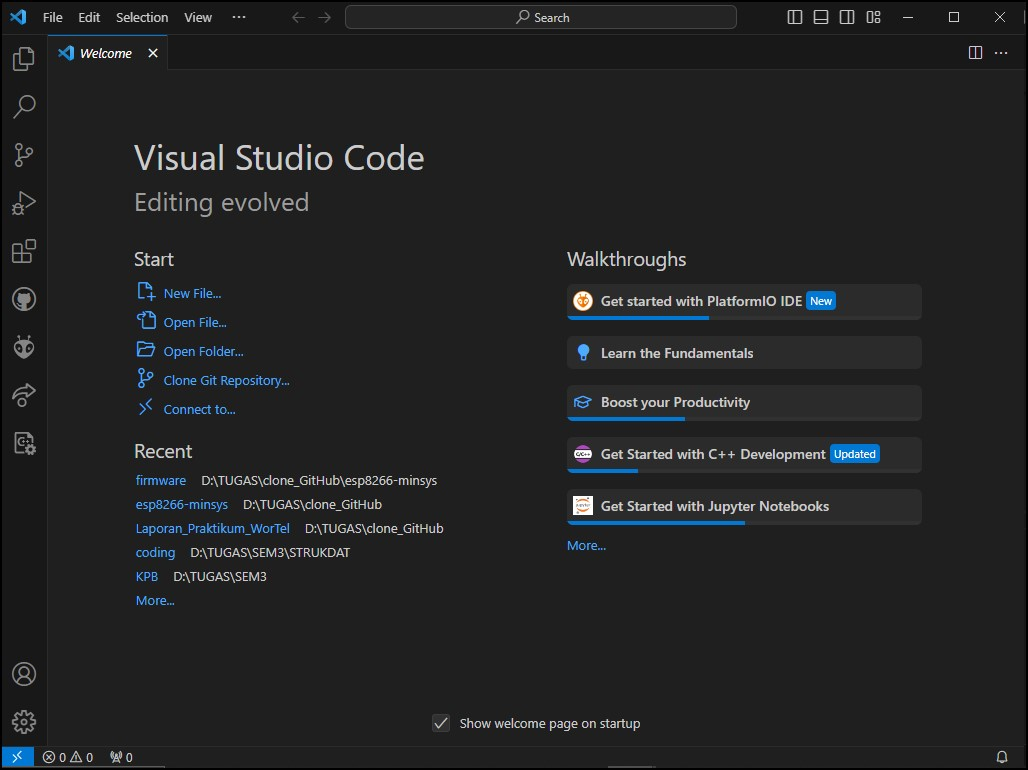
\includegraphics[width=0.6\linewidth]{img/modul_4/tupen_install_vscode.jpg}
    \caption{Bukti install VS Code} 
  \end{figure}
  \item Install ekstensi PlatformIO pada Visual Studio Code
  \begin{figure}[H]
    % Kalau mau menambah gambar lagi tinggal nambahin begin{subfigure} -> end{subfigure}
    \centering
    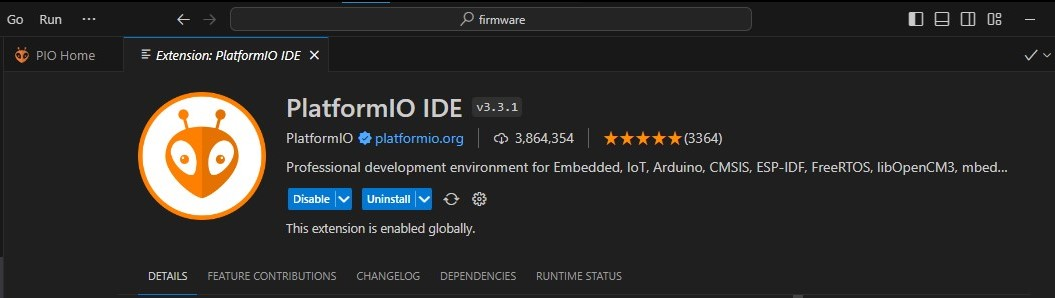
\includegraphics[width=0.9\linewidth]{img/modul_4/tupen_install_platformIO.jpg}
    \caption{Bukti install ekstensi PlatformIO \label{fig:inisub1}}
  \end{figure}
  \item Download firmware dari https://its.id/m/wortel-firmware lalu build project menggunakan vscode + Platformio sampai sukses
  \begin{figure}[H]
    \centering
    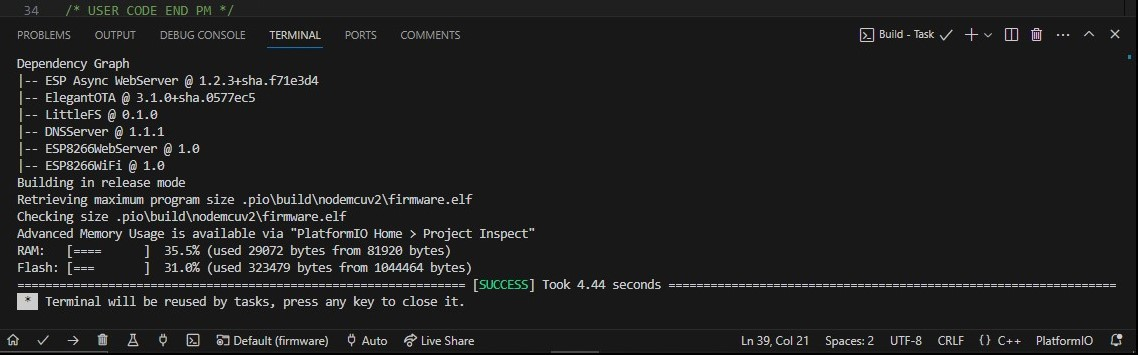
\includegraphics[width=0.9\linewidth]{img/modul_4/tupen_build_platformIO.jpg}
    \caption{Bukti sukses build project dengan platformIO \label{fig:inisub1}}
  \end{figure}
  \item Bukalah https://its.id/m/wortel-simulasi berikut lalu buat program untuk menghidupkan lampu ketika tombol ditekan

  \begin{lstlisting}[language=C++, caption= Kode yang disimulasikan]
  #define LED_RED 5
  #define LED_GREEN 16
  #define LED_BLUE 17
  #define BUTTON_ 26

  uint8_t led_color_rgb[3]={13 + 128, 13 * 2 + 38, 13 * 3 + 47};

  uint8_t btn_val = 0;

  void set_led_color(){
    analogWrite(LED_RED,led_color_rgb[0]);
    analogWrite(LED_GREEN,led_color_rgb[1]);
    analogWrite(LED_BLUE,led_color_rgb[2]);
  }

  void reset_led_color(){
    analogWrite(LED_RED,0);
    analogWrite(LED_GREEN,0);
    analogWrite(LED_BLUE,0);
  }

  void setup() {
    pinMode(LED_RED, OUTPUT);
    pinMode(LED_GREEN, OUTPUT);
    pinMode(LED_BLUE, OUTPUT);

    pinMode(BUTTON_, INPUT);
  }

  void loop() {
    btn_val = digitalRead(BUTTON_);

    if (btn_val == HIGH) {  // kalo tombol ditekan
      set_led_color();      // Atur warna lampu sesuai nilai yang udah ditentuin
    } else {                // kalo ga ditekan, reset warna lampu
      reset_led_color();
    }

    delay(10); 
  }
  \end{lstlisting}
  
  \begin{figure}[H]
    \centering
    % Kalau mau menambah gambar lagi tinggal nambahin begin{subfigure} -> end{subfigure}
    \begin{subfigure}[c]{0.46\linewidth}
      \centering
      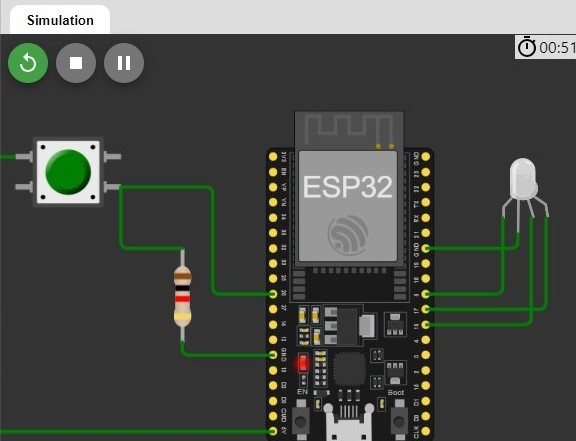
\includegraphics[width=\linewidth]{img/modul_4/tupen_lampu_mati.jpg}
      \caption{Simulasi saat button tidak ditekan (lampu reset) \label{fig:inisub1}}
    \end{subfigure}
    \hspace{1cm}
    \begin{subfigure}[c]{0.46\linewidth}
      \centering
      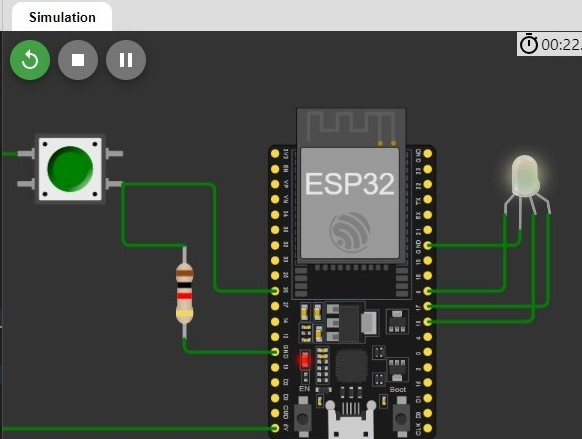
\includegraphics[width=\linewidth]{img/modul_4/tupen_lampu_nyala.jpg}
      \caption{Simulasi saat button ditekan (lampu nyala) \label{fig:inisub2}}
    \end{subfigure}
    \caption{Hasil simulasi \label{fig:keduagambar}}
  \end{figure}
\end{enumerate}
  


% Bagian Analisis Hasil Percobaan
\section*{Analisis Hasil Percobaan}
\indent
Pada workshop telematika modul 3 ini dipelajari tentang cara mendesain 3D sebuah enclosure PCB menggunakan fusion 360. Praktikan diperintahkan untuk membuat enclosure PCB yang terdiri dari minimal enclosure atas dan enclosure bawah serta diharuskan memiliki beberapa lubang pada bagian power, switch, dan beberapa komponen lainnya.  Pada modul dijelaskan secara lengkap mengenai step-step yang harus dilakukan untuk melakukan desain 3D.
\\ \indent 
Setelah desain 3D dilakukan, kemudian praktikan melakukan proses 3D printing menggunakan alat yang telah disediakan di lab AJ403. Sebelum proses 3D printing dilakukan, praktikan diarahkan untuk menggunakan software cura untuk meng export desain 3D ke SD Card untuk kemudian SD Card dimasukkan ke alat 3D printer. Setelah proses export desain selesai lalu dilakukan proses 3D printing.


% \begin{table}[h]
%     \centering
%     \caption{Caption tabelnya}
%     \label{tab:labelini}
%     \begin{tabular}{|c|c|c|c|}
%     \hline
%     Kolom 1 & Kolom 2 & Kolom 3 & Kolom 4 \\
%     \hline
%     Data 1 & Data 2 & Data 3 & coba nambah kolom \\
%     Data 4 & Data 5 & Data 6 & coba nambah kolom juga \\ 
%     \hline
%     \end{tabular}
% \end{table}
% Bagian Lampiran
\section*{Lampiran} % Jika ada lampiran

% ini buat percobaan 1

\begin{figure}[H]
  \centering
  % Kalau mau menambah gambar lagi tinggal nambahin begin{subfigure} -> end{subfigure}
  \begin{subfigure}[c]{0.4\linewidth}
    \centering
    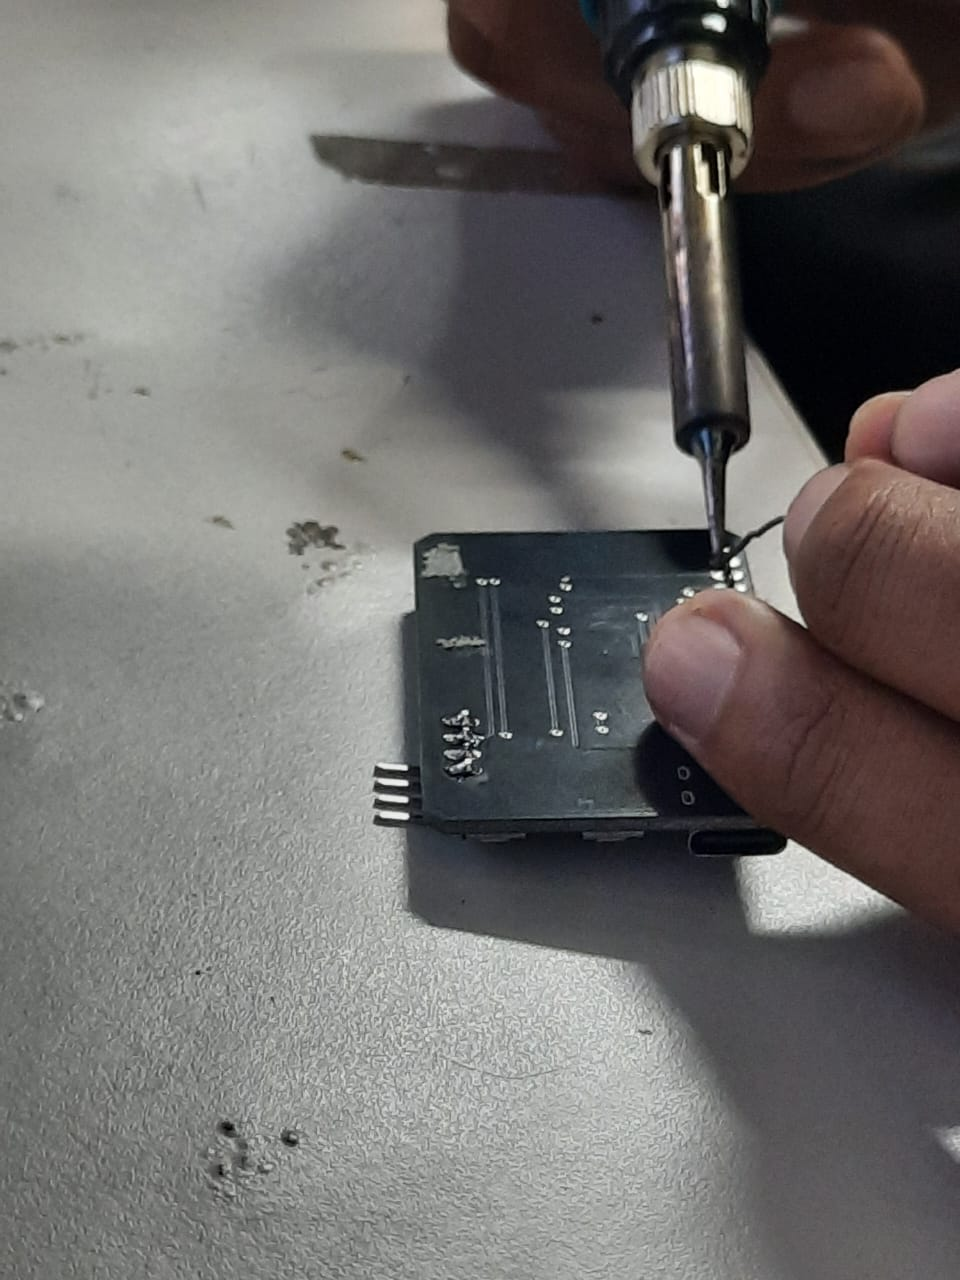
\includegraphics[width=\linewidth]{img/modul_4/proses solder pcb.jpg}
    \caption{Proses peletakan komponen dan soldering PCB\label{fig:inisub1}}
  \end{subfigure}
  \hspace{1cm}
  \begin{subfigure}[c]{0.4\linewidth}
    \centering
    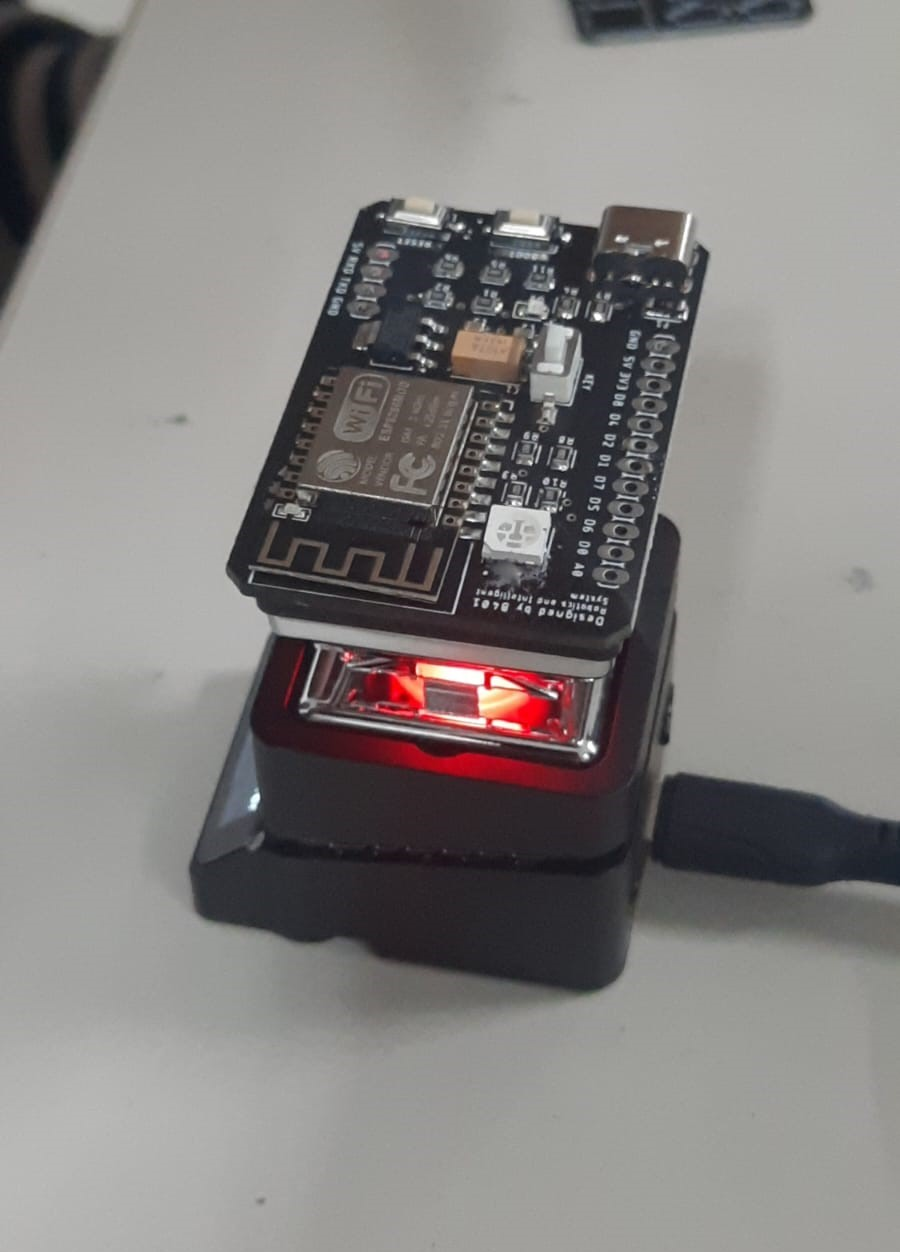
\includegraphics[width=\linewidth]{img/modul_4/proses_pemanasan_pcb.jpg}
    \caption{Proses pemanasan PCB \label{fig:inisub2}}
  \end{subfigure}
  \caption{Proses percobaan \label{fig:keduagambar}}
\end{figure}

\begin{figure}[H]
  \centering
  % Kalau mau menambah gambar lagi tinggal nambahin begin{subfigure} -> end{subfigure}
  \begin{subfigure}[c]{0.4\linewidth}
    \centering
    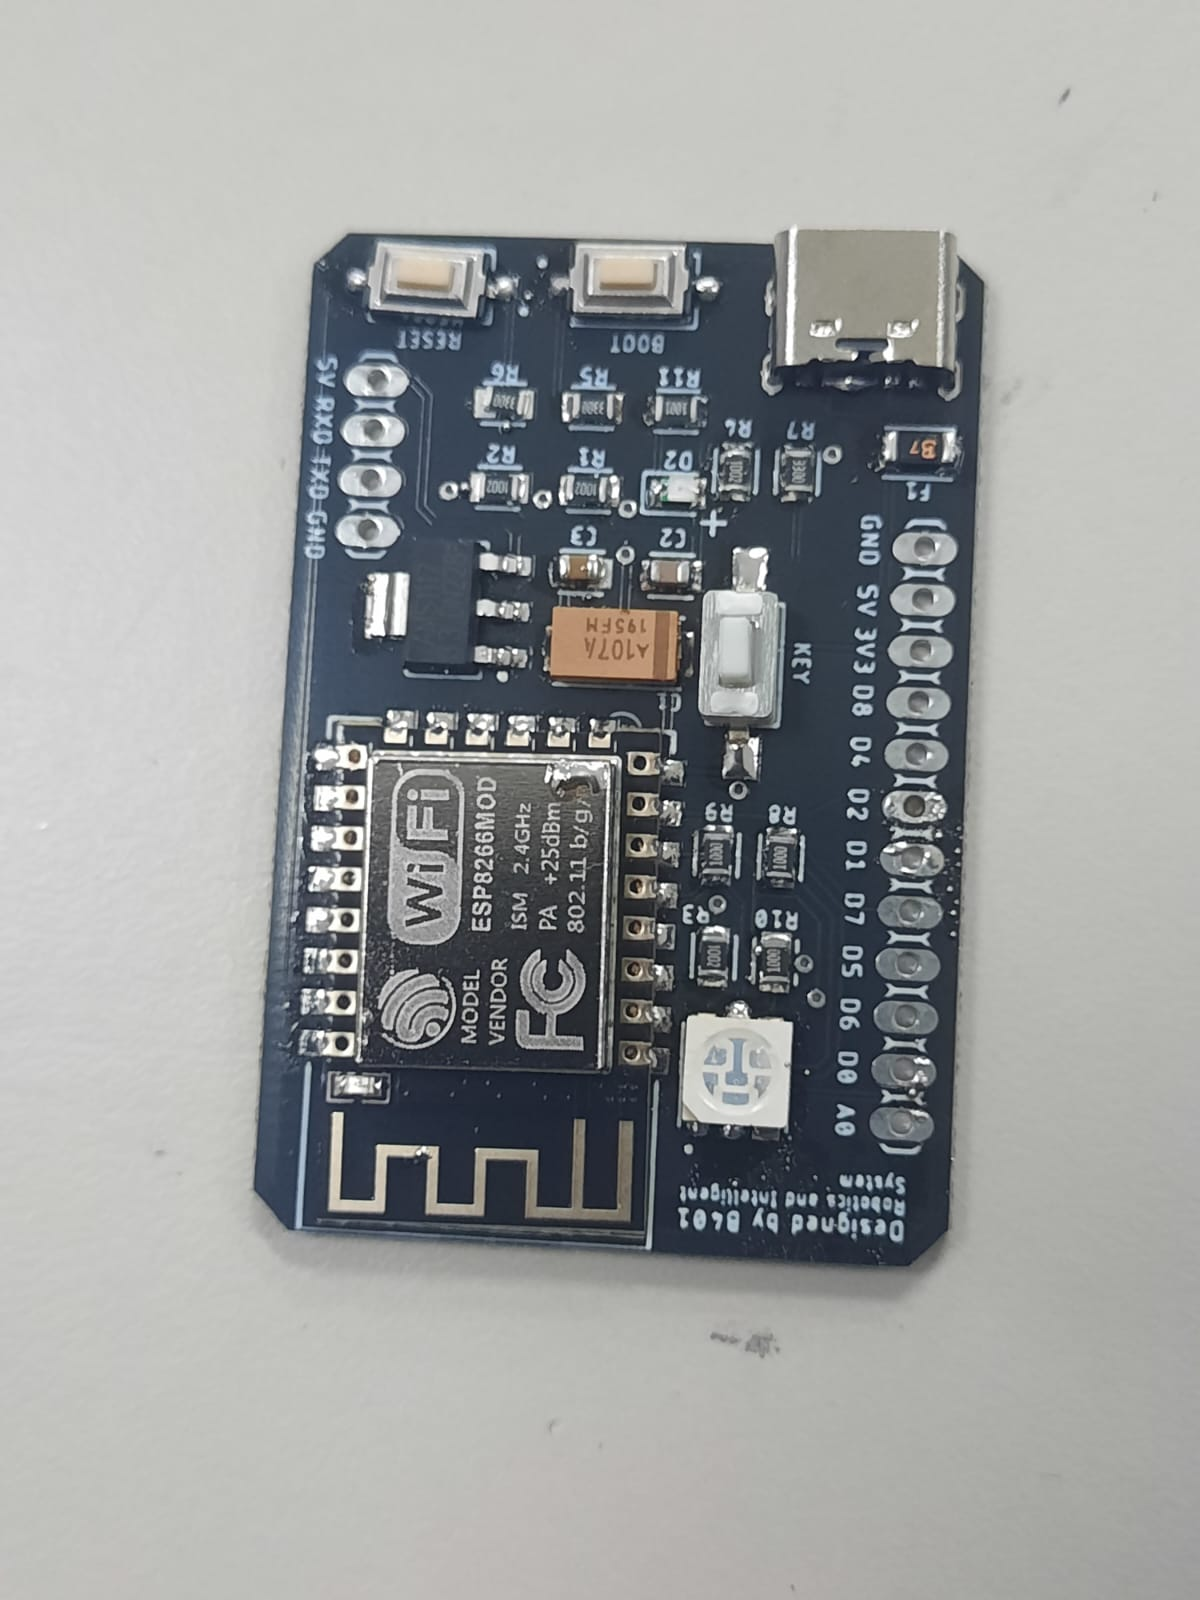
\includegraphics[width=\linewidth]{img/modul_4/hasil_pcb.jpg}
    \caption{Hasil PCB \label{fig:inisub1}}
  \end{subfigure}
  \hspace{1cm}
  \begin{subfigure}[c]{0.4\linewidth}
    \centering
    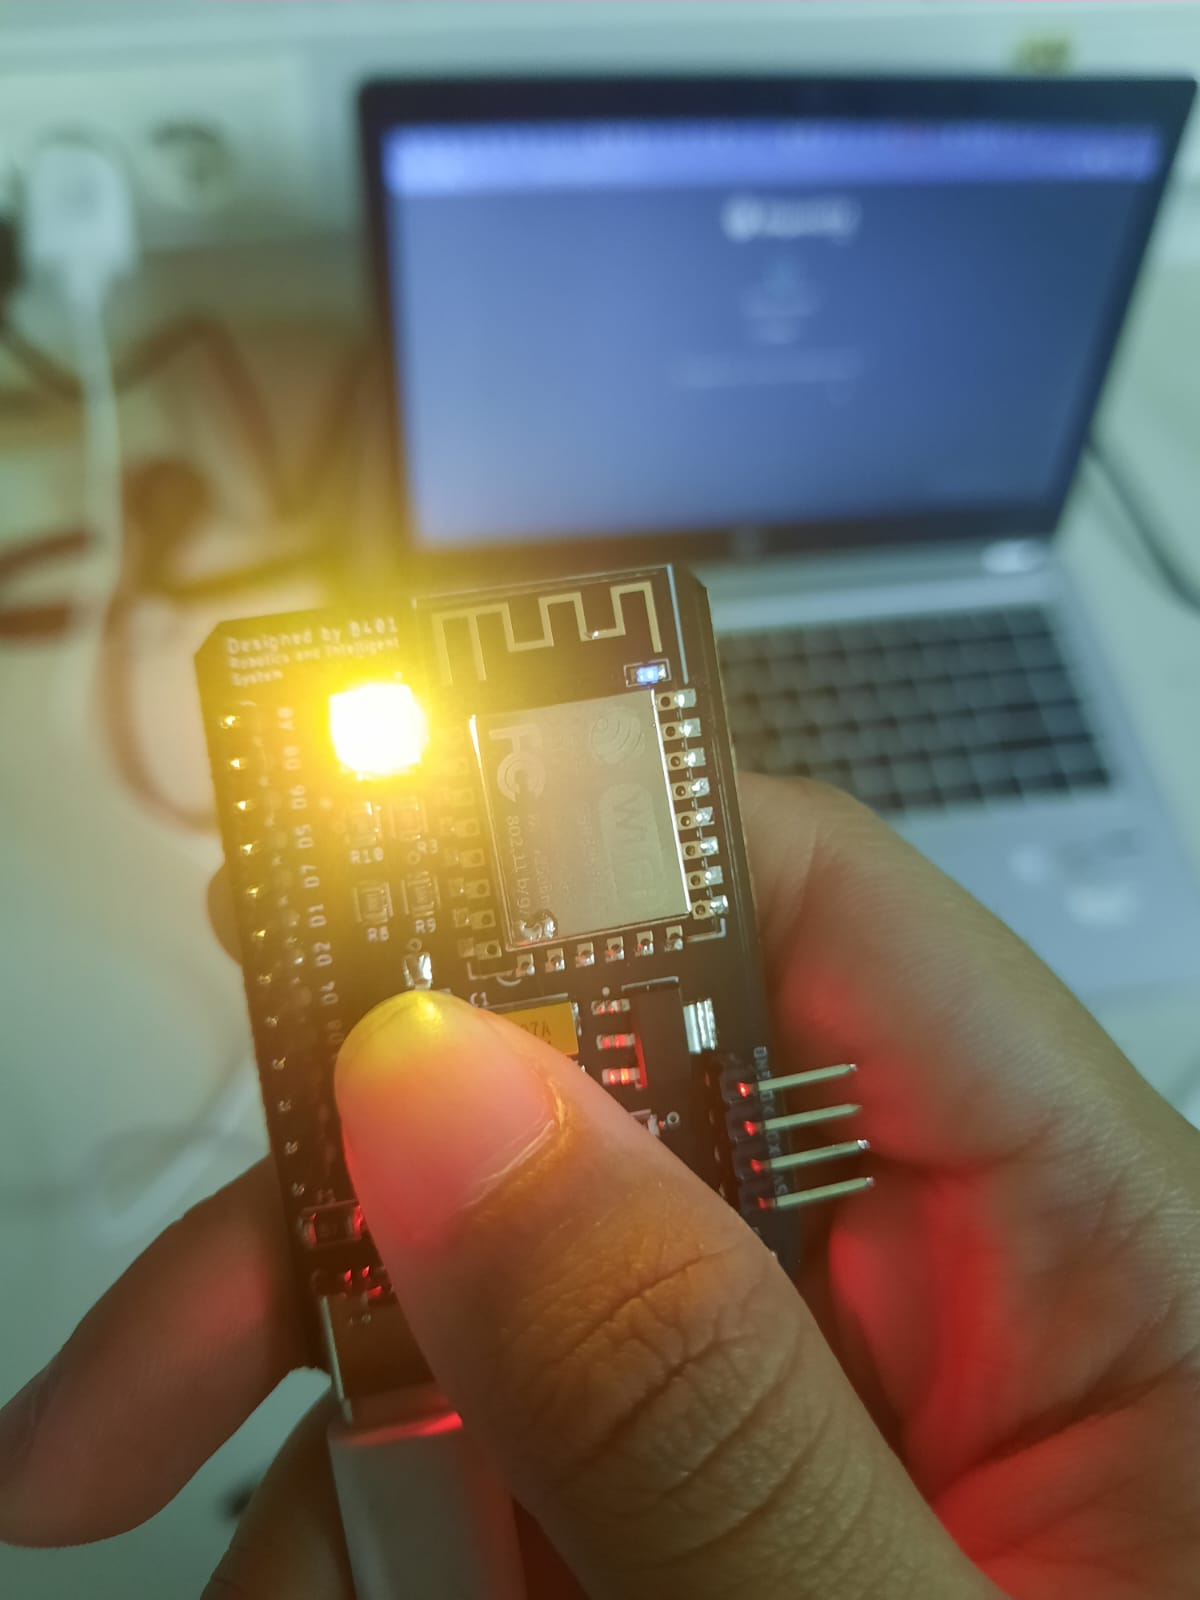
\includegraphics[width=\linewidth]{img/modul_4/hasil_nyala.jpg}
    \caption{Hasil saat LED menyala (button ditekan)\label{fig:inisub2}}
  \end{subfigure}
  \caption*{Hasil percobaan \label{fig:keduagambar}}
\end{figure}
\end{document}